% IEEE Access draft. Compile with the official IEEE Access LaTeX template (ieeeaccess.cls,
% spotcolor.sty, the logo files) copied into this directory; see paper/README.md.
\documentclass{ieeeaccess}
\usepackage{cite}
\usepackage{amsmath,amssymb,amsfonts}
\usepackage[ruled,linesnumbered]{algorithm2e}
\usepackage{graphicx}
\usepackage{textcomp}
\usepackage{booktabs}
\usepackage{xcolor}
\graphicspath{{figures/}}
\newcommand{\todo}[1]{\textcolor{red}{[TODO: #1]}}

\begin{document}
\history{Date of publication xxxx 00, 0000, date of current version xxxx 00, 0000.}
\doi{10.1109/ACCESS.2026.0000000}

\title{How Far Are Learned Multi-AP Schedulers From the Optimum? An Exact-Oracle Gap Analysis of Multi-Agent Reinforcement Learning for IEEE 802.11bn}
\author{\uppercase{Pyoungyun Kim}\authorrefmark{1}, \IEEEmembership{Student Member, IEEE}, and \uppercase{Taeyoon Kim}\authorrefmark{2}}
\address[1]{Visual Display Division, Samsung Electronics, \todo{City Postal code}, Republic of Korea}
\address[2]{School of Mobile System Engineering, Dankook University, \todo{City Postal code}, Republic of Korea}
\tfootnote{\todo{Funding statement}}

\markboth
{P. Kim \emph{et al.}: Exact-Oracle Gap Analysis of Learned Multi-AP Schedulers}
{P. Kim \emph{et al.}: Exact-Oracle Gap Analysis of Learned Multi-AP Schedulers}

\corresp{Corresponding author: Taeyoon Kim (e-mail: \todo{e-mail}).}

\begin{abstract}
Multi-access point coordination (MAPC) in IEEE 802.11bn lets neighboring access points (APs) decide jointly which AP serves which station (STA). Learned schedulers based on multi-agent reinforcement learning (MARL) with centralized training and decentralized execution (CTDE) are usually compared with heuristics whose distance from the optimum is unknown. This paper introduces an exact per-slot oracle that enumerates every joint choice of target STA or silence across APs with the highest decodable modulation and coding scheme (MCS) per link, and uses it to decompose the loss of learned schedulers. Across six topologies and arrival rates from 0.25 to 8 packets per STA per slot, coordinated time division multiple access (Co-TDMA) attains at least 99\% of the oracle up to 2 packets per STA per slot, and the oracle exceeds Co-TDMA by up to 34\% only at high load. A signal-to-interference-plus-noise ratio (SINR) reference that lets all APs transmit attains as little as 25\% of the oracle. At high load and over five training seeds, ideal link adaptation raises proximal policy optimization (PPO) agents by 5--31 percentage points, whereas full information from every AP changes their throughput by $-2$ to $+9$ points. With ideal link adaptation, the learners exceed Co-TDMA by 13--14 points in the two cases with the largest coordination headroom and do not exceed it in any other case. Under per-slot Rayleigh fading, the headroom and the link-adaptation gap grow while the information gap stays within $\pm 5$ points. The bottleneck is therefore rate selection and policy optimization, not inter-AP information.
\end{abstract}

\begin{keywords}
IEEE 802.11bn, multi-access point coordination, multi-agent reinforcement learning, centralized training with decentralized execution, coordinated spatial reuse, link adaptation, Wi-Fi 8.
\end{keywords}

\titlepgskip=-21pt

\maketitle

\section{Introduction}
\label{sec:introduction}
\PARstart{D}{ense} Wi-Fi deployments place several access points (APs) within mutual interference range, so that the throughput of one basic service set depends on the transmission decisions of its neighbors. IEEE 802.11bn, the amendment that defines Wi-Fi~8 with the target of ultra high reliability (UHR), addresses this coupling with multi-access point coordination (MAPC)~\cite{galati2024wifi8}. Under MAPC, APs exchange coordination information and decide jointly whether to share a transmission opportunity (TXOP) in time, as in coordinated time division multiple access (Co-TDMA), or in space, as in coordinated spatial reuse (Co-SR)~\cite{lopez2019ieee}.

Selecting, in every TXOP, the station (STA) each AP serves, whether the AP stays silent, and the modulation and coding scheme (MCS) of every active link is a combinatorial decision over all APs. Multi-agent reinforcement learning (MARL) with centralized training and decentralized execution (CTDE)~\cite{lowe2017maddpg,foerster2018coma,yu2022mappo} is a natural fit: a centralized critic uses the joint observation during training, and each AP executes a local actor that needs no inter-AP message at run time. MARL has been applied to IEEE 802.11bn channel access~\cite{yan2025marl}, and vector quantization (VQ)~\cite{vandenoord2017vqvae} provides a way to bound the size of learned messages exchanged between agents.

The evaluation practice of such schedulers leaves a gap. Learned policies are often compared with random access, greedy rate selection, round-robin scheduling, or a signal-to-interference-plus-noise ratio (SINR) reference that assumes all APs transmit and picks the best MCS for that interference. None of these baselines is an upper bound. Wojnar et~al.~\cite{wojnar2025csr} compute the optimal Co-SR schedule with mixed-integer linear programming and use it as an upper bound for learned scheduling. An optimum alone, however, does not reveal whether the remaining loss of a learned scheduler stems from missing inter-AP information, from rate selection, or from policy optimization.

This paper addresses that question with an exact per-slot oracle and a gap decomposition built on it. The contributions are as follows.
\begin{itemize}
\item An exact per-slot oracle for MAPC scheduling that enumerates all joint (STA or silence) decisions with the highest decodable MCS per link, together with an explicit silence action that lets learned schedulers represent Co-TDMA at all.
\item A load sweep over six reference topologies that quantifies the coordination headroom beyond Co-TDMA and shows that the all-transmit SINR reference attains as little as 25\% of the oracle.
\item A decomposition of the loss of CTDE schedulers based on proximal policy optimization (PPO)~\cite{schulman2017ppo,yu2022mappo} into a link-adaptation gap, an information gap, and a residual optimization gap, obtained by replacing learned MCS selection with automatic rate fallback (ARF)~\cite{kamerman1997arf} or ideal link adaptation, and by contrasting local actors with a full-information actor.
\item An open-source simulator and evaluation suite in which every baseline, learner, and figure of this paper is reproducible from configuration files.
\end{itemize}

The remainder of the paper is organized as follows. Section~\ref{sec:related} reviews related work. Section~\ref{sec:system} defines the system model, and Section~\ref{sec:problem} formulates the scheduling problem. Section~\ref{sec:method} presents the exact oracle, the gap decomposition, and the learners. Section~\ref{sec:setup} details the experimental setup, Section~\ref{sec:results} reports the results, Section~\ref{sec:discussion} discusses their implications and limitations, and Section~\ref{sec:conclusion} concludes the paper.

\section{Related Work}
\label{sec:related}
\subsection{MAPC in IEEE 802.11}
MAPC was studied for IEEE 802.11be and is a core feature of IEEE 802.11bn~\cite{lopez2019ieee,galati2024wifi8}. Co-TDMA divides a TXOP among APs in time, whereas Co-SR lets APs transmit simultaneously and controls the resulting interference through power and rate selection. Wilhelmi et~al.~\cite{wilhelmi2023csr} model IEEE 802.11bn Co-SR with continuous-time Markov chains and report throughput gains of up to 59\% over the legacy distributed coordination function and up to 42\% over the spatial reuse mechanism of IEEE 802.11ax. Nu\~{n}ez et~al.~\cite{nunez2024csr} extend the model of Bianchi to Co-SR in multi-AP networks.

\subsection{MARL for Wi-Fi channel access}
Machine learning, including deep reinforcement learning, has been applied to contention window adaptation, channel bonding, and spatial reuse in Wi-Fi~\cite{szott2022wifiml}. In the CTDE family, the centralized critic of multi-agent deep deterministic policy gradient (MADDPG)~\cite{lowe2017maddpg} and counterfactual multi-agent policy gradients (COMA)~\cite{foerster2018coma}, value factorization as in QMIX~\cite{rashid2018qmix}, and multi-agent PPO (MAPPO)~\cite{yu2022mappo} are standard. Yan et~al.~\cite{yan2025marl} tune the contention window and the clear channel assessment threshold of IEEE 802.11bn channel access with distributed MARL and limit the communication overhead between agents with a fusion network. Learned communication between agents, as in CommNet~\cite{sukhbaatar2016commnet} and TarMAC~\cite{das2019tarmac}, motivates exchanging compact messages between APs, and VQ~\cite{vandenoord2017vqvae} bounds the message size in bits. For MAPC, Nu\~{n}ez et~al.~\cite{nunez2026drl} train a PPO scheduler in an IEEE 802.11bn-compatible environment to minimize the worst-case delay, Yu et~al.~\cite{yu2025hmarl} apply hierarchical MARL to Co-SR, and Wojnar et~al.~\cite{wojnar2025csr} apply machine learning to Co-SR scheduling.

\subsection{Optimality references in learned scheduling}
Reported gains of learned Wi-Fi schedulers are mostly measured against heuristics. Wojnar et~al.~\cite{wojnar2025csr} are an exception: their mixed-integer linear program yields the Co-SR schedule that maximizes throughput or fairness and serves as an upper bound. This paper uses a complementary reference, an exact per-slot oracle over target STA, silence, and MCS under queue dynamics, and decomposes the loss of CTDE learners relative to it. The per-slot problem is tractable for the network sizes of interest because the number of joint decisions grows as the product of the per-AP choice counts.

\section{System Model}
\label{sec:system}
\subsection{Network}
The network consists of $N$ Wi-Fi APs indexed by $i \in \mathcal{N} = \{1,\dots,N\}$. AP $i$ serves the set $\mathcal{S}_i$ of STAs, with $|\mathcal{S}_i| \le K$. Time is divided into scheduling slots of duration $T_{\text{slot}} = 1$~ms, each corresponding to one TXOP. All APs transmit with power $P_{\text{tx}} = 15$~dBm, and the thermal noise power is $P_{\text{N}} = -95$~dBm.

The received power from AP $j$ at a receiver at distance $d$ follows the indoor path-loss model
\begin{equation}
P_{\text{rx}}(d) = P_{\text{tx}} - 46.67 - 30 \log_{10} \max(d, 1) \quad [\text{dBm}].
\label{eq:pathloss}
\end{equation}

\subsection{Traffic and queues}
Each STA $k \in \mathcal{S}_i$ has a downlink queue $q_{i,k}(t) \in [0, Q_{\max}]$ with $Q_{\max} = 100$ packets. In every slot, $A_{i,k}(t) \sim \text{Poisson}(\lambda)$ packets arrive before transmission, which yields the backlog $\tilde{q}_{i,k}(t) = \min\bigl(q_{i,k}(t) + A_{i,k}(t), Q_{\max}\bigr)$. The queue evolves as
\begin{equation}
q_{i,k}(t+1) = \tilde{q}_{i,k}(t) - D_{i,k}(t),
\label{eq:queue}
\end{equation}
where $D_{i,k}(t)$ is the number of packets delivered to STA $k$ in slot $t$. Arrivals occur only at STAs that exist in the topology.

\subsection{Actions}
In slot $t$, AP $i$ selects a target $u_i(t) \in \mathcal{S}_i \cup \{\varnothing\}$, where $\varnothing$ denotes silence, and an MCS index $m_i(t) \in \{0,\dots,M-1\}$ with $M = 16$. The set of transmitting APs is $\mathcal{A}(t) = \{ i : u_i(t) \ne \varnothing,\ \tilde{q}_{i,u_i(t)}(t) > 0 \}$.

\subsection{Interference and link outcome}
The SINR of the link from AP $i$ to STA $k = u_i(t)$ is
\begin{equation}
\gamma_{i}(t) = \frac{P_{\text{rx}}(d_{i,k})}{g(t) \sum_{j \in \mathcal{A}(t) \setminus \{i\}} P_{\text{rx}}(d_{j,k}) + P_{\text{N}}},
\label{eq:sinr}
\end{equation}
where all powers are in linear scale and $g(t) \ge 1$ is an interference gain. The gain equals 1 in the first half of each episode and $g_{\text{h}} = 5$ in the second half, which models a degraded interference regime. In the fading variant of the model, every received power in~\eqref{eq:sinr} is multiplied by an independent power gain $h_{j,k}(t) \sim \text{Exp}(1)$ per transmitting AP $j$, receiving STA $k$, and slot $t$, i.e., Rayleigh block fading with a coherence time of one slot. MCS $m$ requires an SINR of at least $\theta_m = 2 + 1.5m$~dB and carries $c_m = 1 + \lfloor 1.5 m \rfloor$ packets per slot. Some STAs lie in the overlap region of several APs; the set $\mathcal{O}_{i,k}$ lists the APs whose coverage overlaps STA $k$ of AP $i$. A transmission to such a STA fails whenever any AP in $\mathcal{O}_{i,k}$ transmits in the same slot. The delivered packets are therefore
\begin{equation}
D_{i,k}(t) = \mathbb{1}\bigl[\gamma_i(t) \ge \theta_{m_i(t)},\ \mathcal{O}_{i,k} \cap \mathcal{A}(t) = \varnothing\bigr] \min\bigl(\tilde{q}_{i,k}(t), c_{m_i(t)}\bigr),
\label{eq:delivery}
\end{equation}
for $k = u_i(t)$ and $i \in \mathcal{A}(t)$, and $D_{i,k}(t) = 0$ otherwise.

\subsection{Observations}
At the start of slot $t$, AP $i$ observes the local vector
\begin{equation}
o_i(t) = \bigl[\boldsymbol{\beta}_i(t),\ \boldsymbol{\gamma}^{0}_i,\ \boldsymbol{\omega}_i,\ \bar{r}_i,\ \tau(t)\bigr] \in \mathbb{R}^{3K+2},
\label{eq:obs}
\end{equation}
where $\boldsymbol{\beta}_i(t)$ holds the normalized queue lengths $q_{i,k}(t)/Q_{\max}$, $\boldsymbol{\gamma}^{0}_i$ holds the interference-free signal-to-noise ratios (SNRs) of the links normalized by 40~dB, $\boldsymbol{\omega}_i$ holds per-STA overlap indicators, $\bar{r}_i$ is the normalized mean received power from neighboring APs, and $\tau(t)$ indicates the interference regime. Entries of absent STAs are zero. In the fading variant, $\boldsymbol{\gamma}^{0}_i$ holds the mean SNRs and $o_i(t)$ does not contain the fading gains $h_{j,k}(t)$. The joint observation is $\mathbf{o}(t) = [o_1(t),\dots,o_N(t)]$.

\section{Problem Formulation}
\label{sec:problem}
The slot throughput of the joint decision $(\mathbf{u}, \mathbf{m}) = (u_1,\dots,u_N,m_1,\dots,m_N)$ is
\begin{equation}
R(\mathbf{u}, \mathbf{m}; t) = \sum_{i \in \mathcal{A}(t)} D_{i,u_i}(t).
\label{eq:slot_throughput}
\end{equation}
The scheduling objective over an episode of $T$ slots is to maximize the expected cumulative throughput
\begin{equation}
J(\pi) = \mathbb{E}_{\pi}\Bigl[\sum_{t=0}^{T-1} R\bigl(\mathbf{u}(t), \mathbf{m}(t); t\bigr)\Bigr],
\label{eq:objective}
\end{equation}
where $\pi$ maps observations to joint decisions. Under CTDE, $\pi$ factorizes into local actors $\pi_i(u_i, m_i \mid o_i)$ that run at the APs, while a centralized critic $V_\phi(\mathbf{o})$ that uses the joint observation exists only during training. The problem is a decentralized partially observable Markov decision process~\cite{oliehoek2016dec}: no AP observes the queues, the decisions, or the realized interference of the other APs at execution time.

\section{Exact Oracle, Gap Decomposition, and Learners}
\label{sec:method}
\subsection{Exact per-slot oracle}
For a fixed target vector $\mathbf{u}$, the transmitting set $\mathcal{A}(t)$ and hence every SINR in~\eqref{eq:sinr} are determined, because the MCS choice does not change interference. The throughput-maximizing MCS of each link is therefore the highest index whose threshold the link SINR meets,
\begin{equation}
m_i^{\star}(\mathbf{u}) = \max\{ m : \theta_m \le \gamma_i(t) \},
\label{eq:best_mcs}
\end{equation}
and the joint problem reduces to a search over $\mathbf{u}$ alone. The oracle enumerates every $\mathbf{u} \in \prod_{i} (\mathcal{S}_i^{+} \cup \{\varnothing\})$, where $\mathcal{S}_i^{+}$ contains the STAs of AP $i$ with a non-empty backlog $\tilde{q}_{i,k}(t)$, and returns
\begin{equation}
\mathbf{u}^{\star}(t) = \arg\max_{\mathbf{u}} R\bigl(\mathbf{u}, \mathbf{m}^{\star}(\mathbf{u}); t\bigr).
\label{eq:oracle}
\end{equation}
The oracle observes $\tilde{q}_{i,k}(t)$, i.e., the arrivals of slot $t$, and is therefore a genie reference that no causal scheduler matches. For the topologies of this paper, the search covers at most 54 target vectors per slot. At $\lambda = 5$, a Python reference implementation on a single core of a 2.8~GHz Intel Xeon processor takes 1.3~ms per slot in T5 (at most 24 vectors), 3.0~ms in T3 (36 vectors), and 5.8~ms in T6 (54 vectors) on average, with 95th percentiles of 1.6, 3.9, and 7.2~ms. These times exceed the slot duration, so the oracle serves as an offline reference and not as a deployable scheduler. Algorithm~\ref{alg:oracle} summarizes the procedure.

\begin{algorithm}
\caption{Exact per-slot oracle}
\label{alg:oracle}
\KwIn{backlogs $\tilde{q}_{i,k}(t)$, interference gain $g(t)$, overlap sets $\mathcal{O}_{i,k}$}
\KwOut{targets $\mathbf{u}^{\star}(t)$ and MCS indices $\mathbf{m}^{\star}(t)$}
$R^{\star} \leftarrow -1$\;
\ForEach{$\mathbf{u} \in \prod_i (\mathcal{S}_i^{+} \cup \{\varnothing\})$}{
  $\mathcal{A} \leftarrow \{ i : u_i \ne \varnothing \}$\;
  \ForEach{$i \in \mathcal{A}$}{
    compute $\gamma_i$ by~\eqref{eq:sinr} and $m_i^{\star}(\mathbf{u})$ by~\eqref{eq:best_mcs}\;
  }
  $R \leftarrow R(\mathbf{u}, \mathbf{m}^{\star}(\mathbf{u}); t)$ by~\eqref{eq:delivery} and~\eqref{eq:slot_throughput}\;
  \If{$R > R^{\star}$}{
    $R^{\star} \leftarrow R$; $\mathbf{u}^{\star} \leftarrow \mathbf{u}$; $\mathbf{m}^{\star} \leftarrow \mathbf{m}^{\star}(\mathbf{u})$\;
  }
}
\Return{$\mathbf{u}^{\star}, \mathbf{m}^{\star}$}\;
\end{algorithm}

The oracle maximizes the throughput of each slot given the current backlog. Over an episode, the cumulative arrivals $\sum_t \sum_{i,k} A_{i,k}(t)$ plus the initial backlog form a strict upper bound on~\eqref{eq:objective}, and the oracle is reported together with this arrival bound.

\subsection{Reference schedulers}
Co-TDMA activates one AP per slot in round-robin order over the APs with a non-empty backlog; the active AP serves its longest queue with the highest MCS that the interference-free SNR supports. The all-transmit SINR reference lets every AP transmit to its longest non-overlap queue with the highest MCS decodable when all APs transmit. Greedy and round-robin schedulers select the longest queue or cycle through STAs at every AP and adapt the MCS by ARF, which raises the MCS after 10 consecutive successes and lowers it after 2 consecutive failures or after a failed probe~\cite{kamerman1997arf}.

\subsection{Learned schedulers}
Both learners extend the target set of every AP with the silence action $\varnothing$; without it, a learned scheduler transmits whenever its selected queue is non-empty and cannot represent Co-TDMA. The 0-bit learner is MAPPO~\cite{yu2022mappo}: AP $i$ executes a local actor $\pi_{\theta_i}(u_i, m_i \mid o_i)$, and a centralized critic $V_\phi(\mathbf{o})$ is used only for training. The full-information learner (Central PPO) executes a single actor on $\mathbf{o}$ that selects the targets and MCS indices of all APs autoregressively, so that the decision of AP $i$ conditions on the decisions of APs $1,\dots,i-1$. Both learners are trained with PPO~\cite{schulman2017ppo} and generalized advantage estimation~\cite{schulman2016gae} on the normalized slot throughput $R/(10N)$.

\subsection{Gap decomposition}
Let $\Theta^{\star}$ denote the episode throughput of the oracle and $\Theta_{b,\ell}$ that of a learner with information level $b \in \{0, \infty\}$ and MCS control $\ell \in \{\text{learned}, \text{ARF}, \text{ideal}\}$. Under ideal control, the MCS of every transmitting AP equals $m_i^{\star}(\mathbf{u})$ for the targets that the learner selects, so the learner decides only $\mathbf{u}$. With $\rho_{b,\ell} = \Theta_{b,\ell}/\Theta^{\star}$, the loss of a learner decomposes into the link-adaptation gap $\Delta_{\text{LA}} = \rho_{b,\text{ideal}} - \rho_{b,\text{learned}}$, the information gap $\Delta_{\text{I}} = \rho_{\infty,\ell} - \rho_{0,\ell}$, and the residual optimization gap $\Delta_{\text{opt}} = 1 - \rho_{\infty,\text{ideal}}$. The coordination headroom of the network itself is $H = 1 - \Theta_{\text{Co-TDMA}}/\Theta^{\star}$. The two learners differ both in the information available to the actor and in the joint, autoregressive selection of the decisions of all APs. $\Delta_{\text{I}}$ therefore measures the combined value of full information and joint action selection, and it bounds the value of information exchange alone from above.

\section{Experimental Setup}
\label{sec:setup}
Six reference topologies are evaluated. T1 and T2 place three APs on a line with 20~m spacing and one STA per AP; T2 re-indexes T1 and yields identical results. T3 places four APs on a 30~m square grid with two overlap STAs. T4 uses the same grid with one STA per AP and no overlap. T5 clusters four APs at 10~m pitch, with AP~1 serving two STAs. T6 arranges four APs in a T-shape with three overlap STAs, one of which overlaps three APs. Every AP has $K = 4$ target slots, and absent STAs are masked. Fig.~\ref{fig:topologies} shows the six topologies.

\begin{figure*}
\centering
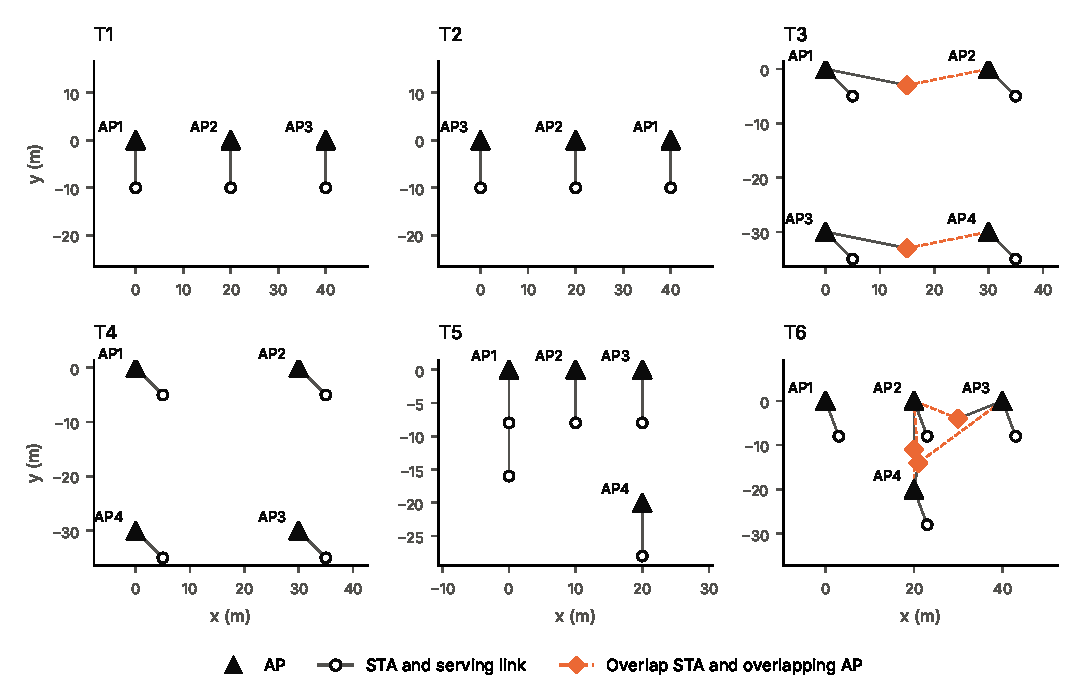
\includegraphics[width=0.9\textwidth]{fig_topologies}
\caption{Reference topologies T1--T6. Solid lines connect each STA to its serving AP; dashed lines connect each overlap STA to the APs whose coverage it overlaps.}
\label{fig:topologies}
\end{figure*}

An episode lasts $T = 200$ slots, and the degraded interference regime starts at slot 100. Arrival rates range over $\lambda \in \{0.25, 0.5, 1, 2, 3, 5, 8\}$ packets per STA per slot. Evaluation uses three seeds per configuration with identical arrival sequences across schedulers.

Both learners use two-layer actors and critics with 128 hidden units and hyperbolic tangent activations. Each PPO update uses four episodes (800 transitions), four epochs over four minibatches, a clip ratio of 0.2, a discount factor of 0.99, a generalized advantage estimation parameter of 0.95, a learning rate of $3 \times 10^{-4}$ with linear decay, and an entropy coefficient of 0.01 with linear decay. Learners train for 1000 episodes with five seeds per configuration and are evaluated with both the most probable action (argmax) and sampled actions. Learner evaluation covers T1 and T3--T6 at $\lambda \in \{5, 8\}$.

\section{Results}
\label{sec:results}
\subsection{Coordination headroom}
Fig.~\ref{fig:headroom}(a) shows that Co-TDMA attains at least 99\% of the oracle in all topologies up to $\lambda = 2$, where the oracle itself attains at least 98\% of the arrival bound. In this regime the network delivers almost every arriving packet, and the only coordination required is to avoid simultaneous transmissions that fail. The headroom $H$ opens at high load: at $\lambda = 5$, the oracle exceeds Co-TDMA by 25\% in T3, 12\% in T5, and 10\% in T6, and at $\lambda = 8$ the gap reaches 34\% in T3 and 30\% in T4. These gains come from Co-SR, i.e., simultaneous transmissions of APs whose links tolerate the mutual interference.

Fig.~\ref{fig:headroom}(b) shows that the all-transmit SINR reference is not an upper bound. It attains 100\% of the oracle in the sparse topology T4 at low and moderate load but only 25--59\% in T5 and 36--57\% in T6 across all loads, because forcing every AP to transmit removes the option of silence.

\begin{figure}
\centering
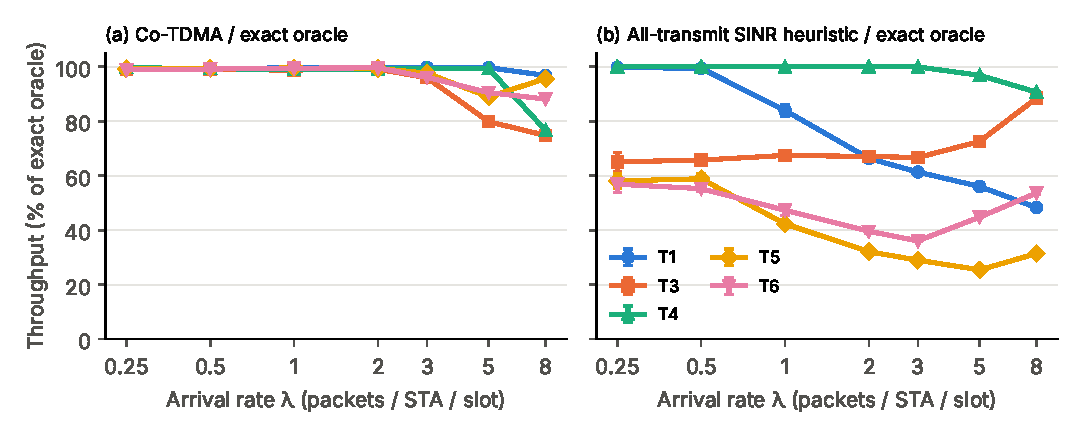
\includegraphics[width=\columnwidth]{fig_headroom}
\caption{Throughput relative to the exact per-slot oracle versus the arrival rate, mean over three seeds with standard deviation. (a) Co-TDMA. (b) All-transmit SINR reference. T2 coincides with T1 and is omitted.}
\label{fig:headroom}
\end{figure}

\subsection{Gap decomposition of learned schedulers}
Table~\ref{tab:load5} reports all schedulers at $\lambda = 5$ as mean and standard deviation over five seeds, with sampled actions for the learners. At this load the headroom $H$ is 0.3\% in T1, 20.5\% in T3, 0.7\% in T4, 11.3\% in T5, and 9.7\% in T6, so T1 and T4 act as controls in which Co-TDMA is already optimal.

\begin{table*}
\caption{THROUGHPUT AS PERCENTAGE OF THE EXACT ORACLE AT $\lambda = 5$ (MEAN $\pm$ STANDARD DEVIATION OVER FIVE SEEDS, SAMPLED ACTIONS FOR LEARNERS)}
\label{tab:load5}
\centering
\begin{tabular}{lccccc}
\toprule
Scheduler & T1 & T3 & T4 & T5 & T6 \\
\midrule
Co-TDMA & 99.7 $\pm$ 0.1 & 79.5 $\pm$ 1.0 & 99.3 $\pm$ 0.1 & 88.7 $\pm$ 0.9 & 90.3 $\pm$ 0.6 \\
All-transmit SINR heuristic & 56.1 $\pm$ 0.4 & 72.1 $\pm$ 1.0 & 97.0 $\pm$ 0.4 & 25.5 $\pm$ 0.4 & 44.6 $\pm$ 0.4 \\
MAPPO (0-bit), MCS learned & 61.0 $\pm$ 5.9 & 57.6 $\pm$ 1.8 & 69.4 $\pm$ 4.2 & 56.6 $\pm$ 1.9 & 51.6 $\pm$ 2.3 \\
MAPPO (0-bit), MCS ARF & 63.8 $\pm$ 3.8 & 61.0 $\pm$ 2.1 & 83.0 $\pm$ 1.9 & 48.8 $\pm$ 3.6 & 48.5 $\pm$ 1.9 \\
MAPPO (0-bit), MCS ideal & 84.6 $\pm$ 1.4 & 74.9 $\pm$ 1.6 & 97.6 $\pm$ 1.1 & 65.6 $\pm$ 4.0 & 66.7 $\pm$ 3.9 \\
Central PPO, MCS learned & 74.5 $\pm$ 9.8 & 58.4 $\pm$ 1.8 & 66.0 $\pm$ 2.5 & 61.0 $\pm$ 2.5 & 52.2 $\pm$ 2.1 \\
Central PPO, MCS ARF & 87.6 $\pm$ 12.7 & 56.7 $\pm$ 4.4 & 82.6 $\pm$ 4.8 & 65.0 $\pm$ 2.0 & 60.3 $\pm$ 13.0 \\
Central PPO, MCS ideal & 92.5 $\pm$ 3.0 & 77.8 $\pm$ 2.9 & 97.4 $\pm$ 0.9 & 71.9 $\pm$ 4.5 & 67.8 $\pm$ 4.4 \\

\bottomrule
\end{tabular}
\end{table*}

Three observations follow from Table~\ref{tab:load5}. First, the link-adaptation gap $\Delta_{\text{LA}}$ is the largest controllable loss: ideal MCS control raises MAPPO by 23.6, 17.3, 28.2, 9.0, and 15.1 percentage points and Central PPO by 18.0, 19.4, 31.4, 10.9, and 15.6 points in T1, T3, T4, T5, and T6. ARF does not substitute for ideal control; its effect on MAPPO ranges from $-7.8$ points in T5 to $+13.6$ points in T4. Second, the information gap $\Delta_{\text{I}}$ under ideal MCS control is 7.9, 2.9, $-0.2$, 6.3, and 1.1 points, i.e., at most 8 points. Third, the residual optimization gap $\Delta_{\text{opt}}$ is 7.5\%, 22.2\%, 2.6\%, 28.1\%, and 32.2\%. The full-information learner with ideal link adaptation therefore does not exceed Co-TDMA in any topology. It falls short of Co-TDMA by 7.2, 1.9, 16.8, and 22.5 points in T1, T4, T5, and T6, with $t$-statistics of the five per-seed differences between $-10.3$ and $-3.8$ (four degrees of freedom, $p < 0.05$). In T3 it is 1.7 points below Co-TDMA, a difference that is not significant ($t = -0.93$).

The argmax policy of the 0-bit learner falls below its sampled policy and varies strongly across seeds (e.g., $51.7 \pm 17.9$\% versus $65.6 \pm 4.0$\% in T5 with ideal MCS control). Local actors with no shared state and nearly constant observations at saturation select the same action at every AP under argmax execution, and randomization is their only mechanism for time sharing.

Table~\ref{tab:load8} repeats the evaluation at $\lambda = 8$, where the headroom $H$ is 3.2\% in T1, 25.1\% in T3, 23.5\% in T4, 4.4\% in T5, and 11.6\% in T6. The link-adaptation gap persists: ideal MCS control raises MAPPO by 18.7, 18.9, 27.4, 7.8, and 16.1 points and Central PPO by 23.4, 16.0, 21.9, 5.4, and 10.2 points in T1, T3, T4, T5, and T6, while the effect of ARF on MAPPO ranges from $-12.1$ points in T5 to $+11.9$ points in T4. The information gap under ideal MCS control is 9.3, 0.8, 0.0, $-1.2$, and $-2.3$ points. In T3 and T4, the two cases with the largest headroom in this study, the learners with ideal MCS control exceed Co-TDMA: MAPPO by 12.6 and 14.1 points and Central PPO by 13.4 and 14.1 points, which corresponds to 53\% and 60\% of the headroom for Central PPO ($t = 13.6$ and $16.3$ over five seeds). In T1, T5, and T6, Central PPO with ideal MCS control stays 11.1, 22.2, and 12.5 points below Co-TDMA ($t$ between $-13.1$ and $-3.1$).

\begin{table*}
\caption{THROUGHPUT AS PERCENTAGE OF THE EXACT ORACLE AT $\lambda = 8$ (MEAN $\pm$ STANDARD DEVIATION OVER FIVE SEEDS, SAMPLED ACTIONS FOR LEARNERS)}
\label{tab:load8}
\centering
\begin{tabular}{lccccc}
\toprule
Scheduler & T1 & T3 & T4 & T5 & T6 \\
\midrule
Co-TDMA & 96.8 $\pm$ 0.5 & 74.9 $\pm$ 0.5 & 76.5 $\pm$ 0.4 & 95.6 $\pm$ 0.2 & 88.4 $\pm$ 0.4 \\
All-transmit SINR heuristic & 48.4 $\pm$ 0.3 & 88.9 $\pm$ 0.6 & 90.7 $\pm$ 0.1 & 31.4 $\pm$ 0.3 & 53.9 $\pm$ 0.4 \\
MAPPO (0-bit), MCS learned & 57.7 $\pm$ 5.7 & 68.6 $\pm$ 3.4 & 63.3 $\pm$ 5.2 & 66.8 $\pm$ 1.6 & 62.1 $\pm$ 1.7 \\
MAPPO (0-bit), MCS ARF & 63.8 $\pm$ 2.5 & 70.6 $\pm$ 2.1 & 75.2 $\pm$ 2.5 & 54.7 $\pm$ 0.8 & 54.5 $\pm$ 5.0 \\
MAPPO (0-bit), MCS ideal & 76.4 $\pm$ 1.0 & 87.5 $\pm$ 1.6 & 90.6 $\pm$ 1.6 & 74.5 $\pm$ 4.6 & 78.2 $\pm$ 3.6 \\
Central PPO, MCS learned & 62.3 $\pm$ 5.0 & 72.3 $\pm$ 6.9 & 68.7 $\pm$ 10.5 & 68.0 $\pm$ 3.1 & 65.6 $\pm$ 5.9 \\
Central PPO, MCS ARF & 64.9 $\pm$ 2.5 & 65.6 $\pm$ 8.2 & 73.1 $\pm$ 4.4 & 72.6 $\pm$ 12.6 & 69.9 $\pm$ 8.6 \\
Central PPO, MCS ideal & 85.7 $\pm$ 7.2 & 88.3 $\pm$ 2.1 & 90.6 $\pm$ 1.4 & 73.4 $\pm$ 3.3 & 75.9 $\pm$ 2.4 \\

\bottomrule
\end{tabular}
\end{table*}

\subsection{Training convergence}
Fig.~\ref{fig:curves} shows the training throughput of the learners in T3 and T6. With ideal MCS control, both learners reach their final level within about 100 episodes in T3, whereas in T6 their throughput rises slowly up to the last episodes. With learned MCS selection, the throughput still rises at 1000 episodes. Across the five topologies, two loads, and five seeds, the mean throughput of episodes 900--999 exceeds that of episodes 500--599 by 9.7\% on average (at most 24.4\%) for MAPPO and by 9.6\% (at most 29.3\%) for Central PPO with learned MCS selection, against 2.5\% (at most 10.4\%) and 4.9\% (at most 23.1\%) with ideal MCS control. The link-adaptation gap $\Delta_{\text{LA}}$ is therefore measured at a fixed budget of 1000 training episodes and overestimates the gap of fully converged learners, The information gap $\Delta_{\text{I}}$ under ideal MCS control compares converged learners in T3 and learners at the same training budget in T6.

\begin{figure}
\centering
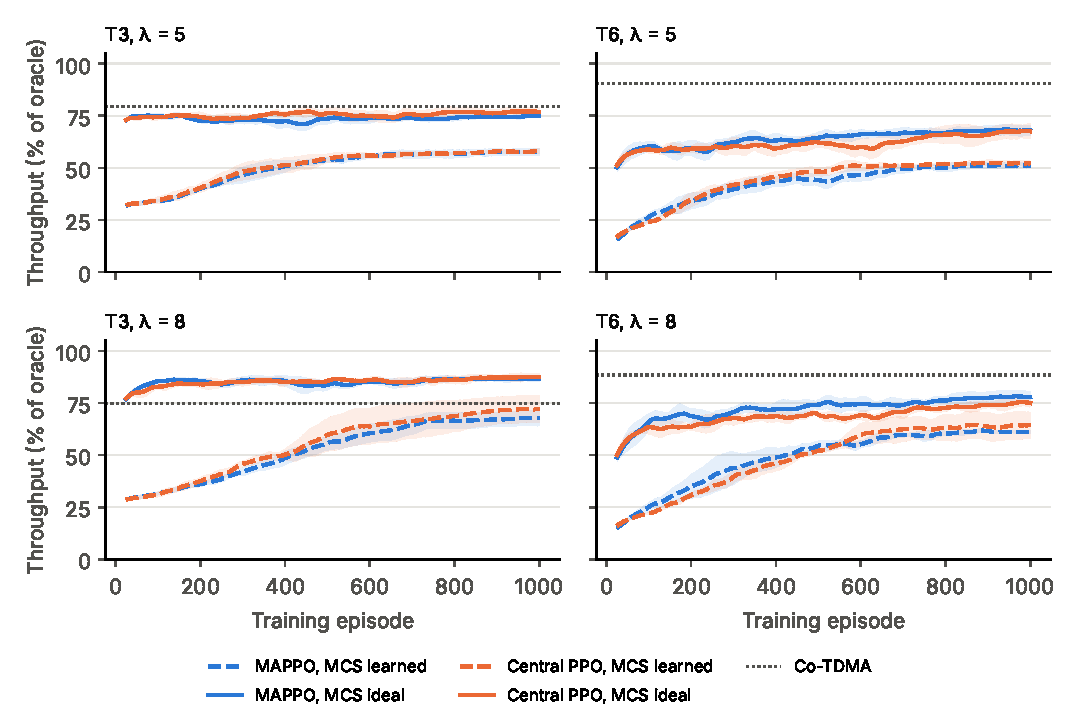
\includegraphics[width=\columnwidth]{fig_learning_curves}
\caption{Training throughput of the learners relative to the mean exact oracle on the evaluation seeds, as a 25-episode moving average with mean and standard deviation over five seeds. Dashed lines denote learned MCS selection, solid lines ideal MCS control, and dotted lines Co-TDMA.}
\label{fig:curves}
\end{figure}

\subsection{Robustness to Rayleigh fading}
Table~\ref{tab:fading} repeats the evaluation for T3 and T6 at $\lambda \in \{5, 8\}$ with Rayleigh block fading and compares it with the deterministic channel over the same three seeds. Fading enlarges the headroom $H$ in all four cases, from 20.2\% to 26.0\% and from 25.2\% to 34.5\% in T3, and from 9.5\% to 21.1\% and from 11.9\% to 27.7\% in T6, because the oracle schedules simultaneous transmissions on links whose instantaneous gain is high. The link-adaptation gap grows as well: ideal MCS control raises MAPPO by 19.4 to 31.5 points under fading against 16.4 to 18.4 points without it, and ARF changes the throughput of MAPPO by $-6.5$ to $+0.5$ points. The information gap under ideal MCS control remains between $-2.0$ and $+4.7$ points. With ideal MCS control, Central PPO exceeds Co-TDMA by 10.1 points in T3 at $\lambda = 8$, is 1.0 point above it in T3 at $\lambda = 5$, and stays 19.0 and 6.5 points below it in T6 at $\lambda = 5$ and $\lambda = 8$. The ordering of the gaps and the conclusions of the deterministic channel therefore hold under fading.

\begin{table*}
\caption{THROUGHPUT AS PERCENTAGE OF THE EXACT ORACLE WITHOUT / WITH RAYLEIGH BLOCK FADING (MEAN OVER THREE SEEDS, SAMPLED ACTIONS FOR LEARNERS)}
\label{tab:fading}
\centering
\begin{tabular}{lcccc}
\toprule
Scheduler & T3, $\lambda = 5$ & T6, $\lambda = 5$ & T3, $\lambda = 8$ & T6, $\lambda = 8$ \\
\midrule
Co-TDMA & 79.8 / 74.0 & 90.5 / 78.9 & 74.8 / 65.5 & 88.1 / 72.3 \\
All-transmit SINR heuristic & 72.6 / 68.5 & 44.8 / 44.9 & 88.5 / 78.3 & 53.7 / 49.3 \\
MAPPO (0-bit), MCS learned & 58.1 / 50.8 & 50.9 / 39.8 & 70.2 / 45.1 & 61.3 / 42.5 \\
MAPPO (0-bit), MCS ideal & 74.5 / 70.3 & 69.0 / 61.9 & 88.6 / 76.6 & 79.7 / 62.0 \\
Central PPO, MCS learned & 59.6 / 52.0 & 52.6 / 41.8 & 72.3 / 45.4 & 66.2 / 41.7 \\
Central PPO, MCS ideal & 79.3 / 75.0 & 71.0 / 59.9 & 87.2 / 75.6 & 76.7 / 65.8 \\

\bottomrule
\end{tabular}
\end{table*}

\section{Discussion}
\label{sec:discussion}
The results separate two questions that evaluations of learned MAPC schedulers commonly merge. The first concerns the network: up to moderate load, Co-TDMA is within 1\% of the oracle, so a learned scheduler cannot demonstrate a coordination gain there, and evaluations at such loads measure the ability to avoid failed simultaneous transmissions. The second concerns the learner: at high load the headroom is real, and the tested PPO learners with ideal link adaptation realize part of it only where it is large: they exceed Co-TDMA in T3 and T4 at $\lambda = 8$, where the headroom is 25.1\% and 23.5\%, and do not exceed Co-TDMA in any other evaluated case. In T3 at $\lambda = 5$, with a headroom of 20.5\%, Central PPO with ideal link adaptation remains 1.7 points below Co-TDMA.

These findings set the agenda for learned inter-AP messages. An information gap of at most 9 percentage points across both loads bounds what any message exchange contributes to the present learners, whereas the link-adaptation and optimization gaps are larger. Measuring the throughput of learned schedulers as a function of the message size in bits is meaningful only after the full-information learner approaches the oracle.

Several remedies target the dominant gaps. First, the action can be decomposed so that the learner selects only the targets and silence, while a classical link-adaptation algorithm, or a separate learned module trained on link outcomes, selects the MCS; the ideal-control results bound the gain of this split, and the ARF results show that the rate-selection component needs to account for the interference that the joint schedule creates. Second, the exact oracle supplies optimal joint actions for every visited state, so imitation learning from the oracle, followed by reinforcement-learning fine tuning with causal observations, offers a direct path to reducing the optimization gap. Third, a curriculum over load, starting at arrival rates where Co-TDMA is near optimal and moving to saturation, exposes the learner to time sharing before it has to discover spatial reuse. Finally, the learned-MCS variants have not converged after 1000 episodes, so longer training reduces part of the link-adaptation gap, although the ideal-control learners show that it does not close the optimization gap at the current budget.

The study has limitations. The oracle is exact per slot but myopic across slots, and it observes the arrivals of the current slot. The two channel models bracket the time variation of indoor channels: deterministic path loss does not vary, and the Rayleigh variant redraws every link in every slot, whereas at 6~GHz and a walking speed of 1~m/s the Doppler frequency is about 20~Hz and the coherence time about 20~ms, i.e., about 20 slots. Shadowing is nearly constant over an episode of 200~ms and acts as a change of STA position, which the six topologies partially cover; mobility changes the association over seconds and lies outside the per-episode scheduling problem. In the fading variant, the observation contains the mean SNR only, so the measured information gap reflects the exchange of queue and link statistics and not of instantaneous channel state. The degraded interference regime is a fixed gain, and the learner results cover two high-load operating points with a fixed budget of 1000 training episodes. Both the learners and the oracle maximize throughput only; fairness across STAs, e.g., the Jain index, and packet delay are not reported, and a throughput-optimal schedule can starve STAs with poor links.

\section{Conclusion}
\label{sec:conclusion}
This paper introduced an exact per-slot oracle for IEEE 802.11bn MAPC scheduling and used it to decompose the throughput loss of CTDE schedulers. Co-TDMA attains at least 99\% of the oracle up to 2 packets per STA per slot, and coordination gains of up to 34\% beyond Co-TDMA appear only at high load. The all-transmit SINR reference attains as little as 25\% of the oracle and is not an upper bound. At high load, ideal link adaptation raises PPO learners by 5--31 percentage points, whereas full inter-AP information changes their throughput by at most 9 points; with ideal link adaptation, the learners exceed Co-TDMA only in the two cases with the largest coordination headroom. These conclusions hold under per-slot Rayleigh fading, which enlarges both the headroom and the link-adaptation gap. Future learned schedulers therefore benefit more from better rate selection and policy optimization than from richer inter-AP messages.

\section*{Acknowledgment}
\todo{Acknowledgment.}

\bibliographystyle{IEEEtran}
\bibliography{references}

\begin{biography}[{\includegraphics[width=1in,height=1.25in,clip,keepaspectratio]{photo/kpy.jpg}}]{Pyoungyun Kim} (S'25)
received the B.S. and M.S. degrees from Korea University, Seoul, Korea, in 2005 and 2007, respectively. Since 2007, he has been with Samsung Electronics, where he has contributed to smart recommendation agents, the integration of the Consumer Electronics Control (CEC) protocol into television systems, and Tizen-based TV software applications. He is currently a Senior Engineer with the Product S/W Lab, Visual Display Division, Samsung Electronics, where he works on multi-view features for smart TVs and screen control for projectors. His research interests include on-device artificial intelligence (AI) for smart displays, embedded deep learning optimization, and resource-efficient deep reinforcement learning (DRL).
\end{biography}

\begin{biography}[{\includegraphics[width=1in,height=1.25in,clip,keepaspectratio]{a.eps}}]{Taeyoon Kim}
received the B.S., M.S., and Ph.D. degrees in electronics and computer engineering from Korea University in 2005, 2007, and 2019, respectively. He was a Research Engineer with Hyundai Motors from 2007 to 2010 and an Assistant Professor with Soonchunhyang University from 2019 to 2021. In 2021, he joined Dankook University as an Assistant Professor with the School of Mobile System Engineering. He was a Visiting Researcher with the University of British Columbia in 2017. His research interests include network architectures and protocols for next-generation networks, such as WLAN, 5G, and time-sensitive networking (TSN), and AI-enabled edge intelligence.
\end{biography}

\EOD

\end{document}
